%-------------------------------------------------------------------
% exp functions
%-------------------------------------------------------------------
\begin{Exercise}[title={$e^x$ functions},label=exExpFunctions]
	\Question Use your calculator to evaluate to 5dp 
	\begin{tasks}(4)
	\task $e^{4}$ %$54.59815$ 
\task $2 e^{ -0.7}$ %$0.99317$ 
\task $e^{3.1}$ %$22.19795$ 
\task $e^{e}$ %$15.15426$
	\end{tasks}

\Question Use Desmos to sketch: 
\begin{tasks}(3)
\task $f (x) =e^{ -x}$ 
\task $g (x) =2 e^{0.1 x}$ 
\task $h (x) = -2.1 e^{ -0.12 x}$
\end{tasks}

\Question Find the exponential function $f (x) =a^{x}$ whose graph is given. 
\begin{tasks}(2)
	\task %	$f (x) =3^{x}$ 
	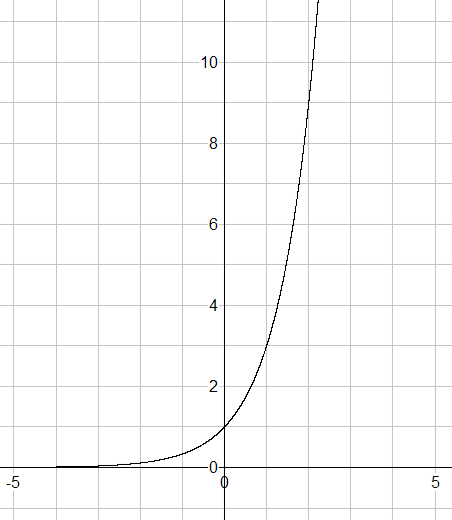
\includegraphics[width=2.3047in, height=2.6472in,]{L4SZ282R}
	
	\task 	%$f (x) =5^{x}$ 
	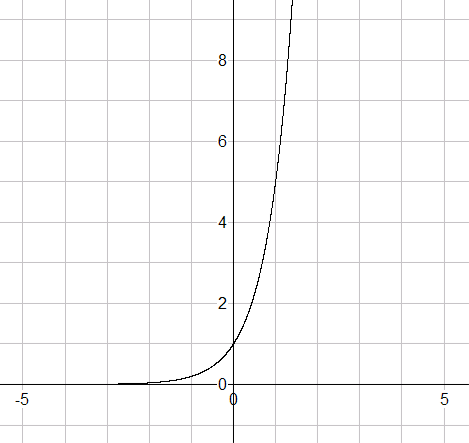
\includegraphics[ width=2.7164in, height=2.5676in,]{L4SZ282S}
	
	\task 	%$f (x) =\genfrac{(}{)}{}{}{1}{4}^{x}$ 
	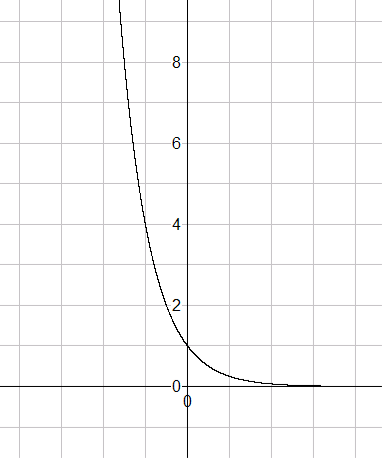
\includegraphics[ width=2.207in, height=2.6394in,]{L4SZ282T}
	
	\task 	%$f (x) =\genfrac{(}{)}{}{}{1}{2}^{x}$ 
	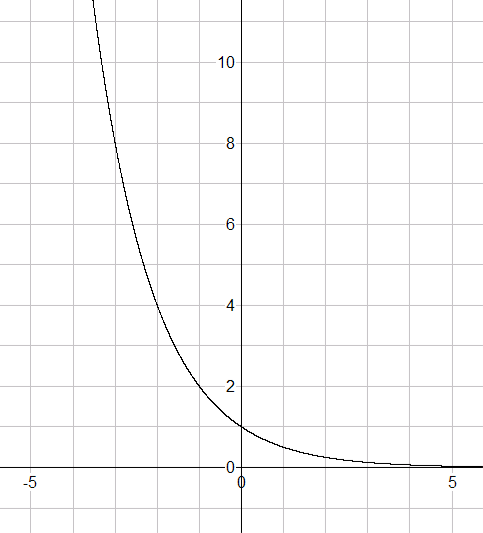
\includegraphics[ width=2.3938in, height=2.6385in,]{L4SZ282U}\\
\end{tasks}

\clearpage
\Question Sketch the transformed graph
\begin{tasks}(2)
	\task The graph is $y =3^x$. \\Draw $y = -3^{x}$.\\ % Use Desmos to verify.
	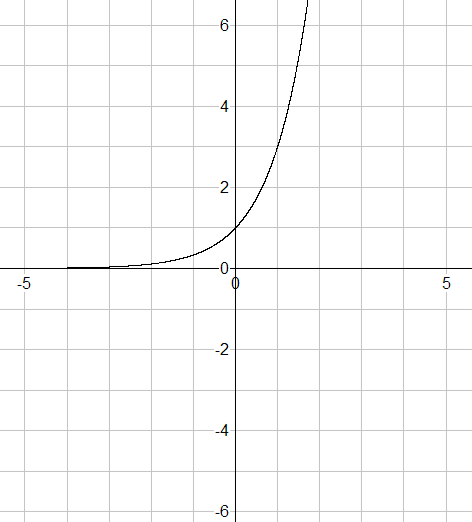
\includegraphics[width=6cm]{L4SZ282V}
	
	\task The graph is $y =2^x$. \\Draw $y =2^{x} -3$.\\% Use Desmos to verify.
	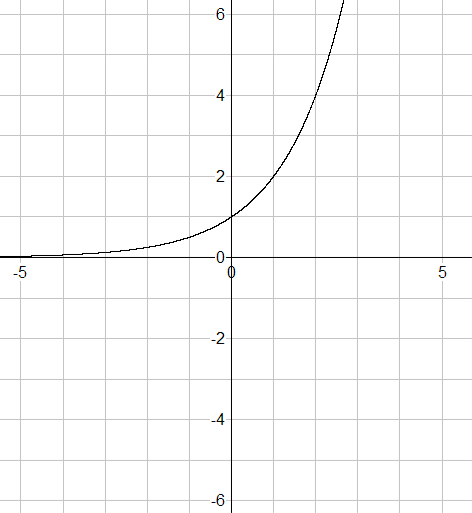
\includegraphics[width=6cm]{L4SZ282W}
	
	\task The graph is $y =\frac{1}{2}^{x}$. \\Draw $y =4 +\frac{1}{2}^{x}$.\\% Use Desmos to verify.
	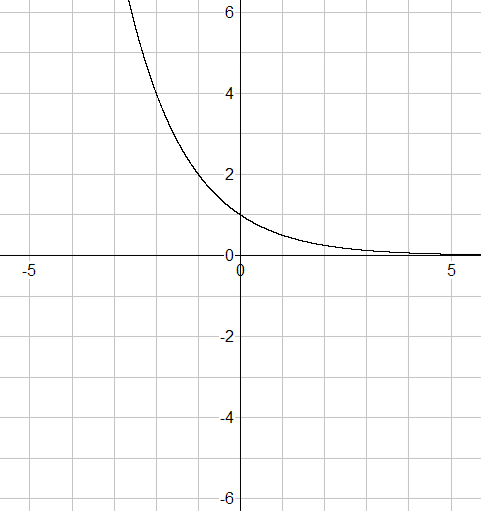
\includegraphics[width=6cm]{L4SZ282X}
	
	\task The graph is $y =10^{x}$. \\Draw $y =10^{x +3}$.\\% Use Desmos to verify.
	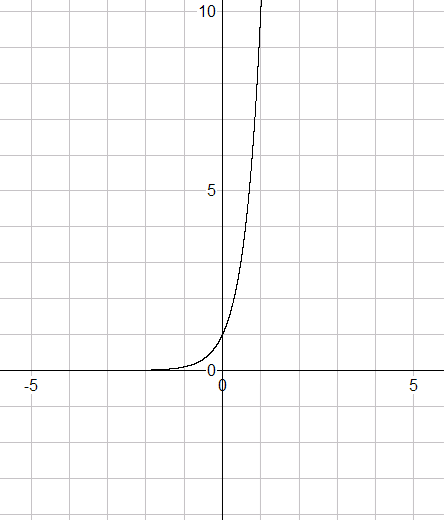
\includegraphics[width=6cm]{L4SZ282Y}
	
	\task The graph is $y =e^{x}$. \\Draw $y = -e^{x}$.\\ % Use Desmos to verify.
	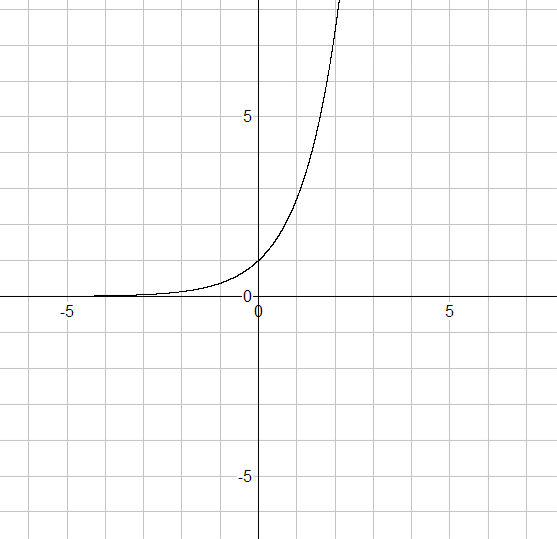
\includegraphics[width=6cm]{L4SZ282Z}
	\task The graph is $y =e^{ -x}$. \\Draw $y =e^{ -x} -1$.\\% Use Desmos to verify.
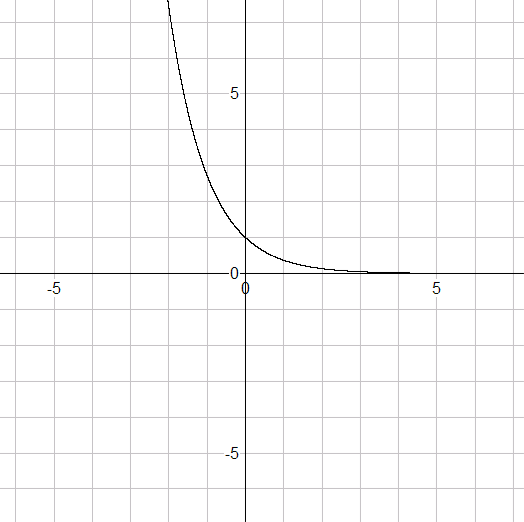
\includegraphics[width=6cm]{L4SZ2830}\\
\end{tasks}
\end{Exercise}
%---------------------------------------------
%--ANSWERS----exp functions-------------------
%---------------------------------------------
\setboolean{firstanswerofthechapter}{true}
\begin{Answer}[ref={exExpFunctions}]
\Question %Use your calculator to evaluate to 5dp 
\begin{tasks}
	\task $54.59815$ 
	\task $0.99317$ 
	\task $22.19795$ 
	\task $15.15426$
\end{tasks}

\Question Use desmos to verify%Use Desmos to sketch: 
%\begin{tasks}
%	\task Use Desmos to verify.%$f (x) =e^{ -x}$ 
%	\task Use Desmos to verify.%$g (x) =2 e^{0.1 x}$ 
%	\task Use Desmos to verify.%$h (x) = -2.1 e^{ -0.12 x}$
%\end{tasks}

\Question %Find the exponential function $f (x) =a^{x}$ whose graph is given. 
\begin{tasks}
	\task $f (x) =3^{x}$ 
	\task $f (x) =5^{x}$ 
	\task $f (x) =\genfrac{(}{)}{}{}{1}{4}^{x}$ 
	\task $f (x) =\genfrac{(}{)}{}{}{1}{2}^{x}$ 
\end{tasks}

\Question Use desmos to verify% Sketch the transformed graph
%\begin{tasks}
%	\task  Use Desmos to verify.
%\task  Use Desmos to verify.
%\task  Use Desmos to verify.
%\task  Use Desmos to verify.
%\task  Use Desmos to verify.
%\task  Use Desmos to verify.
%\end{tasks}	
\end{Answer}%exp functions
\setboolean{firstanswerofthechapter}{false}

%-------------------------------------------------------------------
% log functions
%-------------------------------------------------------------------
\begin{Exercise}[title={Logarithmic Functions},label=exLogFunctions]
	\Question Express the equation in exponential form. 
	\begin{tasks}(3)
		\task  $\log _{5} 25 =2$	%$5^{2} =25$
		\task $\log _{5} 1 =0$	%$5^{0} =1$
		\task $\log _{8} 2 =\frac{1}{3}$	%$8^{1/3} =2$
		\task $\log _{2} \genfrac{(}{)}{}{}{1}{8} = -3$		%$2^{ -3} =\frac{1}{8}$ 
		\task $\ln  5 =x$ 	%$e^{x} =5$
		\task $\ln  y =5$	%$e^{5} =y$ 
	\end{tasks}

	\Question Express the equation in logarithmic form 
\begin{tasks}(3)
	\task  $5^{3} =125$	%$\log _{5} 125 =3$
	\task  $10^{ -4} =0.0001$	%$\log _{10} 0.0001 = -4$
	\task $8^{ -1} =\frac{1}{8}$	%$\log _{8} \frac{1}{8} = -1$
	\task 	$2^{ -3} =\frac{1}{8}$	%$\log _{2} \frac{1}{8} = -3$
	\task $e^{x} =2$	%$\ln  2 =x$
	\task $e^{3} =y$	%$\ln  y =3$ 
\end{tasks}

	
	\Question Evaluate the expression 
	\begin{tasks}(3)
		\task $\log _{3} 3$ %1
		\task $\log _{3} 1$	%0
		\task $\log _{3} 3^{2}$	%2
		\task $\log _{6} 36$	%$2$
		\task $\log _{9} 81$ 	%$2$ 
		\task $\log _{7} 7^{10}$ 	% $10$
		\task $\log _{3} \genfrac{(}{)}{}{}{1}{27}$ 	%$ -3$
		\task $\log _{10} \sqrt{10}$ 	% $\frac{1}{2}$ 
		\task $\log _{5} 0.2$ 	%$ -1$ 
		\task $2^{\log _{2} 37}$ 	%$37$
		\task $3^{\log _{3} 8}$ 	%$8$
		\task $e^{\ln  \sqrt{5}}$	%$\sqrt{5}$
		\task $\log _{8} 0.25$ 	%$ -\frac{2}{3}$
		\task $\ln  e^{4}$ 	%$4$
		\task $\ln  \left (1/e\right )$ 	%$ -1$ 
	\end{tasks}

\Question Use the definition of the logarithmic function to find $x$.
\begin{tasks}(3)
	\task $\log _{2} x =5$ 		%$32$
	\task $\log _{2} 16 =x$ 	%$4$
	\task $\log _{3} 243 =x$ 	%$5$
	\task $\log _{10} x =2$ 	%$100$
	\task $\log _{x} 16 =4$ 	%$2$
	\task $\log _{x} 8 =\frac{3}{2}$ 	%$4$
\end{tasks}
	
\Question Use the Laws of Logarithms to rewrite the expression in a form with no logarithms of products, quotients roots or powers.
\begin{tasks}(3)
	\task $\log _{2} \left (2 x\right )$					%$1 +\log _{2} x$ 
	\task $\log _{2} \left (x \left (x -1\right )\right )$ 	%$\log _{2} x +\log _{2} \left (x -1\right )$ 
	\task $\log  6^{10}$ 							%$10 \log  6$
	\task $\log _{2} \left (A B^{2}\right )$		%$\log _{2} A +2 \log _{2} B$ 
	\task $\log _{3} \left (x \sqrt{y}\right )$		%$\log _{3} x +\frac{1}{2} \log _{3} y$ 
	\task $\log _{5} \sqrt[{3}]{x^{2} +1}$ 		%$\frac{1}{3} \log _{5} \left (x^{2} +1\right )$ 
	\task $\ln  \sqrt{a b}$ 						%$\frac{1}{2} \left (\ln  a +\ln  b\right )$ 
	\task $\ln  \left (x \sqrt{\frac{y}{z}}\right )$	%$\ln  x +\frac{1}{2} \left (\ln  y -\ln  z\right )$ 
	\task $\log  \sqrt[{4}]{x^{2} +y^{2}}$		%$\frac{1}{4} \log  \left (x^{2} +y^{2}\right )$ 
\end{tasks}

\Question Evaluate the expressions
\begin{tasks}(3)
	\task $\log _{5} \sqrt{125}$	%$\frac{3}{2}$
	\task $\log  2 +\log  5$		%$1$
	\task $\log _{4} 192 -\log _{4} 3$	% $3$ 
	\task $\ln  6 -\ln  15 +\ln  20$	%$\ln  8$ 
	\task $10^{2 \log  4}$ 			%$16$
	\task $\log  \left (\log  1000^{10,000}\right )$	%$4 +\log  3$ 
\end{tasks}
	
	\Question Rewrite the expression as a single logarithm
	\begin{tasks}(1)
		\task $\log _{3} 5 +5 \log _{3} 2$	%$\log _{3} 160$ 
		\task $\log _{2} A +\log _{2} B -2 \log _{2} C$%$\log _{2} \left (A B/C^{2}\right )$ 
		\task $\ln  5 +2 \ln  x +3 \ln  \left (x^{2} +5\right )$ %$\ln  \left [5 x^{2} \left (x^{2} +5\right )^{3}\right ]$ 
		\end{tasks}
	

\end{Exercise}	
%---------------------------------------------
%--ANSWERS----log functions-------------------
%---------------------------------------------
\begin{Answer}[ref={exLogFunctions}]
\Question %Express the equation in exponential form. 
\begin{tasks}
	\task  $5^{2} =25$
	\task $5^{0} =1$
	\task $8^{1/3} =2$
	\task $2^{ -3} =\frac{1}{8}$ 
	\task $e^{x} =5$
	\task $e^{5} =y$ 
\end{tasks}

\Question %Express the equation in logarithmic form 
\begin{tasks}
	\task  $\log _{5} 125 =3$
	\task  $\log _{10} 0.0001 = -4$
	\task $\log _{8} \frac{1}{8} = -1$
	\task $\log _{2} \frac{1}{8} = -3$
	\task $\ln  2 =x$
	\task $\ln  y =3$ 
\end{tasks}


\Question %Evaluate the expression 
\begin{tasks}
	\task 1
	\task 0
	\task 2
	\task 2
	\task 2 
	\task 10
	\task $ -3$
	\task $\frac{1}{2}$ 
	\task $ -1$ 
	\task $37$
	\task $8$
	\task $\sqrt{5}$
	\task $ -\frac{2}{3}$
	\task $4$
	\task $ -1$ 
\end{tasks}

\Question %Use the definition of the logarithmic function to find $x$.
\begin{tasks}
	\task $32$
	\task $4$
	\task $5$
	\task $100$
	\task $2$
	\task $4$
\end{tasks}

\Question %Use the Laws of Logarithms to rewrite the expression in a form with no logarithms of products, quotients roots or powers.
\begin{tasks}
	\task $1 +\log _{2} x$ 
	\task $\log _{2} x +\log _{2} \left (x -1\right )$ 
	\task $10 \log  6$
	\task $\log _{2} A +2 \log _{2} B$ 
	\task $\log _{3} x +\frac{1}{2} \log _{3} y$ 
	\task $\frac{1}{3} \log _{5} \left (x^{2} +1\right )$ 
	\task $\frac{1}{2} \left (\ln  a +\ln  b\right )$ 
	\task $\ln  x +\frac{1}{2} \left (\ln  y -\ln  z\right )$ 
	\task $\frac{1}{4} \log  \left (x^{2} +y^{2}\right )$ 
\end{tasks}

\Question %Evaluate the expressions 
\begin{tasks} 
	\task $\frac{3}{2}$
	\task $1$
	\task $3$ 
	\task $\ln  8$ 
	\task $16$
	\task $4 +\log  3$ 
\end{tasks}

\Question %Rewrite the expression as a single logarithm
\begin{tasks}
	\task $\log _{3} 160$ 
	\task $\log _{2} \left (A B/C^{2}\right )$ 
	\task $\ln  \left [5 x^{2} \left (x^{2} +5\right )^{3}\right ]$ 
\end{tasks}


\end{Answer}%log functions
%-------------------------------------------------------------------
% equations
%-------------------------------------------------------------------
\begin{Exercise}[title={Logarithmic Equations},label=exLogEqns]
\Question Find the solution of the exponential equation, correct to four decimal places. 
\begin{tasks}(3)
	\task $e^{x} =16$ 		%$2.7726$
	\task $10^{2 x} =5$ 	%$0.3495$ 
	\task $3 e^{x} =10$ 	%$1.2040$ 
	\task $e^{1 -4 x} =2$ 	%$0.0767$
	\task $8^{0.4 x} =5$ 	%$1.9349$
	\task $5^{ -x/100} =2$	%$ -43.0677$ 
	\task $5^{x} =4^{x +1}$ %	$6.2126$
	\task $2^{3 x +1} =3^{x -2}$ 	%$ -2.9469$ 
	\task $100 \left (1.04\right )^{2 t} =300$	%$14.0055$ 
\end{tasks}

\Question Solve the equations for $x$ 
\begin{tasks}(2)
	\task $x^{2} 2^{x} -2^{x} =0$ %$ \pm 1$
	\task $4 x^{3} e^{ -3 x} -3 x^{4} e^{ -3 x} =0$%$0 ,\frac{4}{3}$ 
	\task $e^{4 x} +4 e^{2 x} -21 =0$ %$\frac{1}{2} \ln  3 \approx 0.5493$
	\task $\ln  x =10$ %$e^{10} \approx 22026$ 
	\task $\log  \left (3 x +5\right ) =2$%$\frac{95}{3}$ 
	\task $2 -\ln  \left (3 -x\right ) =0$%$3 -e^{2} \approx  -4.3891$ 
	\task $\log  x +\log  \left (x -1\right ) =\log  \left (4 x\right )$ %$5$ 
	\task $\log _{5} \left (x +1\right ) -\log _{5} \left (x -1\right ) =2$ %$\frac{13}{12}$ 
\end{tasks}	
\end{Exercise}
%---------------------------------------------
%--ANSWERS----log equations-------------------
%---------------------------------------------
\begin{Answer}[ref={exLogEqns}]
\Question %Find the solution of the exponential equation, correct to four decimal places. 
\begin{tasks}
	\task $2.7726$
	\task $0.3495$ 
	\task $1.2040$ 
	\task $0.0767$
	\task $1.9349$
	\task $ -43.0677$ 
	\task $6.2126$
	\task $ -2.9469$ 
	\task $14.0055$ 
\end{tasks}

\Question %Solve the equations for $x$ 
\begin{tasks}
	\task $ \pm 1$
	\task $0 ,\frac{4}{3}$ 
	\task $\frac{1}{2} \ln  3 \approx 0.5493$
	\task $e^{10} \approx 22026$ 
	\task $\frac{95}{3}$ 
	\task $3 -e^{2} \approx  -4.3891$ 
	\task $5$ 
	\task $\frac{13}{12}$ 
\end{tasks}		
	
\end{Answer}%log equations
%-------------------------------------------------------------------
% modelling
%-------------------------------------------------------------------
\begin{Exercise}[title={Modelling},label=exModelling]
	\Question A radioactive substance decays in such a way that the amount of mass remaining after $t$ days is given by the function
	\begin{equation*}m (t) =13 e^{ -0.015 t}
	\end{equation*} Where $m (t)$ is measured in kilograms. 
	\begin{tasks}
		\task Find the mass at time $t =0$.% $13 \mbox{kg}$
		\task How much of the mass remains after 45 days?% $6.6 \mbox{kg}$ 
	\end{tasks}
	
	\Question A sky diver jumps from a reasonable height above the ground. The air resistance she experiences is proportional to her velocity, and the constant of proportionality is $0.2$. It can be shown that the downward velocity of the sky diver at time $t$ is given by
	\begin{equation*}v (t) =80 \left (1 -e^{ -0.2 t}\right )
	\end{equation*} \\\relax where $t$ is measured in seconds and $v (t)$ is measured in feet per second ($\mbox{ft}$/$\mbox{s}$).
	\begin{tasks}
		\task Find the initial velocity of the sky diver.%$0$
		\task Find the velocity after $5 \mbox{s}$ and after $10 \mbox{s}$. %$50.6 ft/\mbox{s} ,69.2 ft/\mbox{s}$
		\task Draw a graph of the velocity function $v (t)\text{.}$%no graph
		\task The maximum velocity of a falling object with wind resistance is called the \emph{terminal velocity}. From the graph in part (c) find the terminal velocity of the sky diver. %$80 ft/\mbox{s}$
	\end{tasks}

\Question The population of a certain species of bird is limited by the type of habitat required for nesting. The population behaves according to the \emph{logistic growth model}
\begin{equation*}n (t) =\frac{5600}{0.5 +27.5 e^{ -0.044 t}}
\end{equation*}  where $t$ is measured in years.
	\begin{tasks}
	\task Find the initial bird population. %$200$
	\task Draw a graph of the function $n (t)$.%no graph
	\task What size does the population approach as time goes on?%$11,200$
\end{tasks}

\Question A $15 \mbox{g}$ sample of radioactive iodine decays in such a way that the mass remaining after $t$ days is given by $m \left (t\right ) =15 e^{ -0.087 t}$ where $m (t)$ is measured in grams. After how many days is there only $5 \mbox{g}$ remaining? %$13$ days

\Question A small lake is stocked with a certain species of fish. The fish population is modelled by the function
\begin{equation*}P =\frac{10}{1 +4 e^{ -0.8 t}}
\end{equation*} where $P$ is the number of fish in thousands and $t$ is measured in years since the lake was stocked. 
\begin{tasks}
\task Find the fish population after $3$ years. %$7337$
\task After how many years will the fish population reach $5000$ fish? %$1.73 \mbox{y}$r 
\end{tasks}
\end{Exercise}
%---------------------------------------------
%--ANSWERS----modelling-------------------
%---------------------------------------------
\begin{Answer}[ref={exModelling}]
\Question %A radioactive substance decays 
\begin{tasks}
	\task $13 \mbox{kg}$
	\task $6.6 \mbox{kg}$ 
\end{tasks}

\Question %A sky diver jumps from a reasonable height above the ground
\begin{tasks}
	\task $0$ $\frac{\text{ft}}{\text{s}}$
	\task $50.6$  $\frac{\text{ft}}{\text{s}}$, $69.2$ $\frac{\text{ft}}{\text{s}}$
	\task Use desmos to plot the graph
	\task $80$ $\frac{\text{ft}}{\text{s}}$
\end{tasks}

\Question %The population of a certain species of bird is 
\begin{tasks}
	\task $200$
	\task Use desmos to plot the graph
	\task $11,200$
\end{tasks}

\Question %A $15 \mbox{g}$ sample of radioactive iodine decays 
$13$ days

\Question %A small lake is stocked with a certain species of fish. 
\begin{tasks}
	\task $7337$
	\task $1.73$ years 
\end{tasks}
\end{Answer}%modelling

